% Drawing 23/03-2 -- folder 23, batch 03, archive page 59 (PDF page 60).
% Transcription: le dessin « ci-contre », en bas à gauche : un axe horizontal $p$ et un axe vertical $q$, fléchés ; une bande verticale hachurée de largeur $d$, à gauche de l'axe des $q$ et appuyée sur lui, commence à la hauteur $a$ au-dessus de l'axe des $p$ et monte ; la hauteur $a$ et la largeur $d$ sont cotées par des flèches doubles.
% Kind: hatched vertical band in the (p, q) plane (support of E_2^{pq}). Method 2 (schematic redraw from the facsimile). Status: ok.
% Notes: As on the page: the p-axis and the q-axis with their arrowheads and letters; the band between the q-axis and a parallel line at its left, closed below at height a and open above, hatched obliquely; the double arrow marked a from the p-axis up to the foot of the band, at the right of the q-axis; the double arrow marked d under the p-axis, spanning the width of the band. The band's lower edge, its left side and the axis are drawn between the same points. Redrawn 2026-11-12 (issue 128): to check again.
% Coordinates: 1 unit = 1 mm = 1/100 of the crop width (bbox in page fractions: [0.12, 0.72, 0.36, 0.885]).
% Redrawn by Claude (claude-fable-5-2), issue #128, 2026-11-12; not checked by a human; not compiled (no TeX in the session).
% Rights: reproduces part of the work -- behind RENDER_TRANSCRIPTS, never published by itself.
\documentclass[tikz,border=3pt]{standalone}
\usepackage{amsmath,amssymb}
\usetikzlibrary{patterns,arrows.meta}
\tikzset{pencil/.style={black!45}, struck/.style={black!35}, mpt/.style={circle,draw,inner sep=1.3pt}, pt/.style={circle,fill,inner sep=0.9pt}, opt/.style={circle,draw,fill=white,inner sep=1.1pt}}
\begin{document}
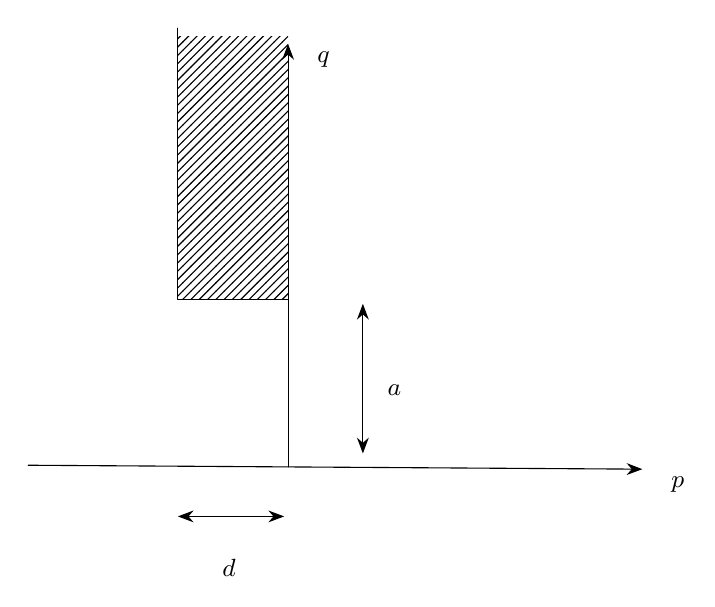
\begin{tikzpicture}[x=1mm,y=1mm,line cap=round,line join=round,font=\scriptsize]
\draw[-{Stealth[length=2mm]}] (0,-71.5) -- (78,-72);
\draw[-{Stealth[length=2mm]}] (33,-71.7) -- (33,-18);
\draw (19,-16) -- (19,-50.5) -- (33,-50.5);
\fill[pattern=north east lines] (19,-17) -- (19,-50.5) -- (33,-50.5) -- (33,-17) -- cycle;
\draw[{Stealth[length=2mm]}-{Stealth[length=2mm]}] (42.5,-51) -- (42.5,-70);
\draw[{Stealth[length=2mm]}-{Stealth[length=2mm]}] (19,-78) -- (32.5,-78);
\node[inner sep=1pt] at (37.5,-20) {\small $q$};
\node[inner sep=1pt] at (82.5,-74) {\small $p$};
\node[inner sep=1pt] at (46.5,-62) {\small $a$};
\node[inner sep=1pt] at (25.5,-84.5) {\small $d$};
\end{tikzpicture}
\end{document}
